%%%%%%%% symbols to add
\simbolo{\eta}{Additive noise function}
\simbolo{\ast}{Convolution operation}
\simbolo{\delta}{Dirac delta function}
\simbolo{\mathbb{R}}{Set of real numbers}
\simbolo{\mathbb{N}}{Set of natural numbers}
\simbolo{\wedge}{Diagonal matrix of decrescent multiple singular values}
\simbolo{\mathbb{G} = (\mathbb{V},\mathbb{E})}{Graph}
\simbolo{\mathbb{V}}{Set of vertices of a graph}
\simbolo{\mathbb{E}}{Set of edges of a graph}

{\color{red}
This chapter aims to provide the necessary image processing background for the blur map construction and the image fusion procedure, as proposed by in the project. The approach for obtaining the blur map is an extension of the segmentation techniques, as they are created and used for extracting regions of interest in images. On the other hand, image fusion comprises a series of methods commonly applied in photography that will be addressed from a scientific point of view. Blur may have different causes such as movement, defocus, aberrations in the optical system, among others. All of them are addressed by researchers with image processing. On the other hand, image fusion can be seen as a decision problem, which can be dealt with a large amount of methods.}

\section{Image formation}
\noindent - image formation - depth of field\\
- details about depth of field\\
- diffraction-limited resolution\\
- finite lens aperture\\
- spectral support\\
- aberrations\\
- resolution limit\\
- defocus blur only\\
- numerical aperture\\

\section{Blur Characterization}

% According to \citeonline{smith2007modern}, every optical system exhibits blur properties, in higher or lower proportions, due to the depth of focus and its adjustment. The defocus blur is caused by the incidence of light within an aperture with significant dimensions, where the source of light is not properly placed in accordance to the focal plane; it is related to the variables of the optical system such as depth of focus, aperture, depth of field, aberrations and so on \cite{joshi2014defocus}. Motion blur is caused by the attempt of taking pictures from moving objects and camera displacements; it can be caused in large scales (an image of a moving runner) or in small scales (live cell imaging). Both types of blur result in a loss of image details, sharpness and information. It can also be classified into global and partial blur. The former consists of a mathematically well-behaved homogeneous process and the latter is related to real world blurring phenomena. In light microscopy applications, the most relevant type is the partial defocus blur. Figure \ref{fig:defocus_motion_blur} shows an example of large scale defocus and motion blurs.

% \begin{figure}[H]
% 	\centering
% 	\caption{\label{fig:defocus_motion_blur}Defocus blur (left) and motion blur (right) in large scales.}
% 	\begin{center}
% 	    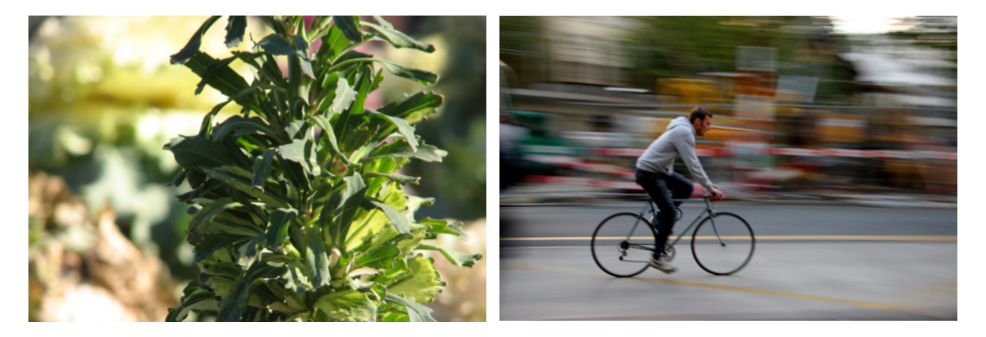
\includegraphics[scale=0.4]{images/fig7.png}
% 	\end{center}
% 	\centering
%     \fadaptada{su2011blurred}
% \end{figure}

% \subsection{Point Spread Function}

% Dirac delta functions are generalized functions designed for representing an impulse - a infinitely high value within a infinitely small period of time \cite{bracewell2000fourier}. In a nutshell, it is a function $\delta(x)$ that is zero-valued for any $x \neq 0$ and is infinity-valued for $x = 0$. This property can be combined with any smooth function $f\colon \mathbb{R}^{n} \to \mathbb{R}^{n}$, given  and provides the property shown in equation \ref{eqn:dirac_delta_function} in low dimension for didactic purposes. Figure \ref{fig:discrete_dirac_delta} illustrates the delta function on  $A = \{\, x\in \mathbb{R} \mid 0\le x\le 10^{7} \,\}$ normalized into the $[0,1]$ interval.

% \begin{equation}
%     \label{eqn:dirac_delta_function}
%       \int^{\infty}_{-\infty}\delta(x-a)f(x) = f(a)
% \end{equation}

% \begin{figure}[H]
% 	\centering
% 	\caption{\label{fig:discrete_dirac_delta}Discrete representation of the Dirac delta function.}
% 	\begin{center}
% 	    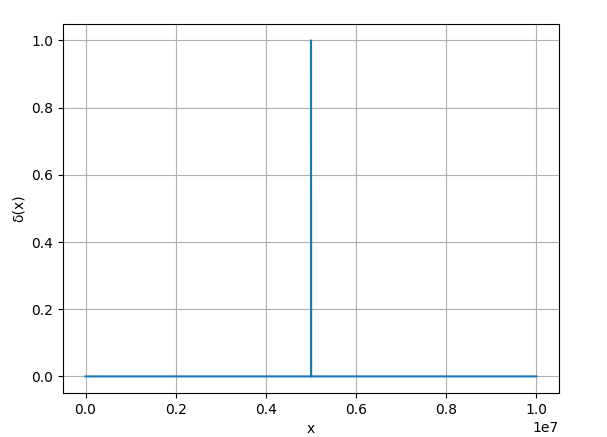
\includegraphics[scale=0.5, trim = {0 0.6cm 0 1.5cm}]{images/fig9.png}
% 	\end{center}
% 	\centering
%     \fautor
% \end{figure}

% This concept of impulse is a light source with the shape of a point when it comes to images. It provides the effect of blurring on images, since it promotes the diffusion of the acquired information. Figure \ref{fig:psf} shows an arbitrary example of a punctual source of light and its image, which suffers the spreading effect.

% \begin{figure}[H]
% 	\centering
% 	\caption{\label{fig:psf}Magnified image of a light impulse (left) and its impulse response function, the PSF (right).}
% 	\begin{center}
% 	    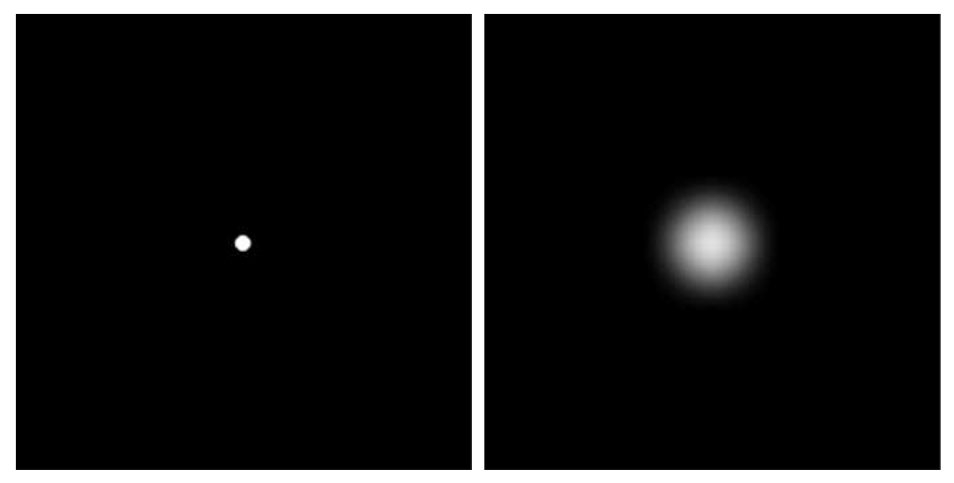
\includegraphics[scale=0.4]{images/fig8.png}
% 	\end{center}
% 	\centering
%     \fadaptada{gonzalez2008digital}
% \end{figure}

% Digital images can be considered as discrete representations of a continuous space, as the image acquisition consists in the action of several sensors that capture light from the environment and divide the information into pixels. Hence, the most trivial and used representation for digital images are matrices of pixels and can be described as functions that suffer the influence of other functions during acquisition. The degradation process which stands for the influence quoted before may be mathematically illustrated by equation \ref{eqn:degradation_model} \cite{gonzalez2008digital}:

% \begin{equation}
%     \label{eqn:degradation_model}
%       g(x,y) = h(x,y) \ast f(x,y) + \eta(x,y)
% \end{equation}

% \noindent where $f(x,y)$ is the function that represents the original image from the scene, $g(x,y)$ is the degraded image, $\eta(x,y)$ is the additive noise function and $h(x,y)$ is the point spread function of the imaging system. The $\ast$ symbol represents the convolution operation: in conformity with \citeonline{bracewell2000fourier}, it is an integral that relates a function $f$ with a function $g$ by means of a weighted sum in the range of a variable $u$, and is denoted by equation \ref{eqn:convolution}:

% \begin{equation}
%     \label{eqn:convolution}
%       \int^{\infty}_{-\infty}f(u)g(x - u)du
% \end{equation}

% Thus, the blurring process can be considered as a natural phenomenon guided by a convolution operation, but it may suffer interference of factors such as motion of the object, the scene or the camera and differences of the surface's topology when it comes to microscopy. 


{\color{red} TRANSFORMS AND FUSION SHOULD BE MOVED TO IMAGE PROCESSING CHAPTER}

% \section{Image Transforms}

% Usually, the most trivial image processing operations are done at the pixel level; they act on one of the channels of an image from an specific color space, on gray levels of a grayscale image and so on. Some procedures such as the convolution have the computational performance as a bottleneck, and this is one of the reasons why \emph{image transforms} are widely used. They encompass any group of mathematical operations that takes the input signal or the input image out of their domain an project them onto the transformed domain \cite{gonzalez2008digital}. The convolution operation, for instance, turns itself into a simple matrix multiplication task on the Fourier Transform domain (which will be detailed in the following sections) and that solves the performance bottleneck. The general structure of a forward image transform and an inverse image transform is denoted by  the pair of equations \ref{eqn:generic_transform}, respectively:


% \begin{align}
%     \label{eqn:generic_transform}
%     T(u,v) = 
%     \sum_{x=0}^{M-1}
%     \sum_{y=0}^{N-1}f(x,y)r(x,y,u,v)
%     &&
%     f(x,y) = 
%     \sum_{x=0}^{M-1}
%     \sum_{y=0}^{N-1}T(u,v)s(x,y,u,v)
% \end{align}

% \noindent where $M$ and $N$ are the dimensions of the image, $x$ and $y$ are coordinates of the image, $u = \{0,1,2,...,M-1\}$ and $v = \{0,1,2,...,N-1\}$ are called transform variables, $r(x,y,u,v)$ is a function named \emph{forward transform kernel} that is responsible for the forward domain change and finally $s(x,y,u,v)$ is the inverse kernel for $r$. These equations take an image to another domain, perform some operations and then return to the spatial domain. These are the common steps in transforms applications indeed. The following sections contain details about relevant image transforms in image segmentation and image fusion.

% \subsection{Fourier Transform}

% The Fourier Transform is a mathematical framework that expresses a periodic or non-periodic function with a sum of weighted sinusoids, what results in a set of different frequencies \cite{gonzalez2008digital}. The transform relies on complex numbers and the Euler's formula. The complex numbers belong to the broadest of the number sets, i.e. $\mathbb{R} \subseteq \mathbb{C}$, and consists of a \emph{real part} $a$ and an \emph{imaginary part} $bj$, shown by equation \ref{eqn:complex_number}:

% \begin{equation}
% \label{eqn:complex_number}
%     z = a + bj
% \end{equation}

% \noindent where $j = \sqrt{-1}$ is the imaginary unit. In this sense, the Euler's formula relates complex exponential functions with trigonometric functions through the equation  \ref{eqn:euler_formula}:

% \begin{equation}
% \label{eqn:euler_formula}
%     e^{j\theta} = \cos{\theta} + j\sin{\theta}
% \end{equation}

% \noindent where $\theta \in \mathbb{R}$ is a number that represents an angle in radians. This is the fundamental framework to describe the Fourier transform, since it is a sum of function representations by means of the Euler's formula. According to \citeonline{brigham1988fast}, the Continuous and the \sigla{DFT}{Discrete Fourier Transform} in a simplified version can be computed as shown on the left and on the right of Equation \ref{eqn:fourier_transform}, respectively:

% \begin{align}
% \label{eqn:fourier_transform}
%     H(x) = \int_{-\infty}^{\infty}h(t)e^{-j2 \pi tx}dt
%     &&
%     H(x) = \sum_{x=0}^{N-1}h(t)e^{-j2 \pi t \frac{x}{N}}
% \end{align}

% \noindent with $H(x)$ as the Fourier transform of a function $h(t)$, $t$ represents functions is the time domain, $x$ represents the frequency domain and $N$ represents the total number of samples on the discrete approach. As already pointed out, images can be interpreted as two-dimensional functions; hence, the most important version of the Fourier transform in the context of image processing is the two-dimensional DFT, given by Equation \ref{eqn:2D_dft}:

% \begin{equation}
% \label{eqn:2D_dft}
%     H(u,v) = \frac{1}{\sqrt{MN}}\sum_{x=0}^{M-1}\sum_{y=0}^{N-1}h(x,y)e^{-j2 \pi \big(\frac{ux}{M} + \frac{vy}{N}\big)}
% \end{equation}

% \noindent where $h(x,y)$ consists of an image, $M$ and $N$ are the image dimensions and $u$ and $v$ are coordinates in the frequency domain. This operation is extremely useful for almost every field related to analysis of functions. However, the DFT consists of a convolution process with $O(n^{2})$ asymptotic complexity, which can be too slow for larger dimensions. The \sigla{FFT}{Fast Fourier Transform} is an algorithm to compute the DFT by taking small slices of the signal, computing the transform with them and them merging the result. This procedure is performed in $O(n \log n)$ complexity, which is reasonable for many applications.


% \section{Image Fusion}

% Immediately upon the blur map extraction is satisfactorily complete, an image fusion operation is needed in order to achieve the highest amount of focused regions as possible. Image fusion is a process that merges several images (possibly taken in diverse conditions or with different cameras) into one image with higher quality, more details and consequently more useful for humans and computer tasks \cite{mitchell2010image}. Image fusion techniques can be used in noise reduction, edge enhancement and super-resolution, for example. 

% One prominent use of image fusion occurs in medical image fields; the quality of information about illnesses, cells, clinical analysis and several other medical tasks (including the computer assisted ones) have found profitable results from the techniques and lead themselves to better and faster decisions when it comes to human beings \cite{james2014medical}.

% There are relevant applications in remote sensing multispectral images, segmentation of regions in different colourspaces, biometry: the pan-sharpening process is the generation of an high resolution multispectral image from low to high resolution ones, K-Means segmentation and fusion of pixels in the \sigla{RGB}{Red, Green and Blue colourspace} and the Iris Recognition biometric process with video frames are examples of such tasks, respectively \cite{mitchell2010image}.

% \subsection{General Framework}

% Still according to \citeonline{mitchell2010image}, the general framework for the image fusion procedure can be accomplished in four stages: Multiple Input Images, Common Representational Format, Fusion and Display.
% The \emph{multiple input images} stage consists in obtaining the set of images which will be merged. There are several approaches to this: the dataset may be captured from different sensors, on distinct light conditions or angles, with different magnifications, on several focus and with temporal measurements if the scene changes through time.

% After the image set generation, there is the necessity of reshaping each item. This configures the \emph{common representational format}, responsible for creating a new and temporary dataset with the same properties, e.g. colourspace, dimensions, noise level and so on. The \emph{fusion} stage consists of using a decision method in order to dictate which regions, objects, colours or details will compose the final image; this can be done by any approach that relates to how the result should be. There are some methods that rely on the Wavelet Transform domain, for example. Finally, the \emph{display} stage consists in providing a view for the resulting image, which can be used directly for any further task or even be the input for other image processing operation. Figure \ref{fig:fusion_general_framework} depicts an arbitrary example of the four stages:

% \begin{figure}[H]
% 	\centering
% 	\caption{\label{fig:fusion_general_framework}Image fusion general framework. (a) Multiple Input Images, (b) Common Representational Format, (c) Fusion and (d) Display.}
% 	\begin{center}
% a 	    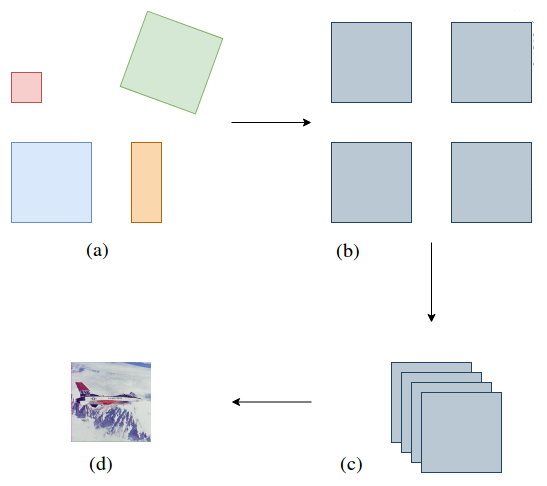
\includegraphics[scale=0.4]{images/fig10.png}
% 	\end{center}
% 	\centering
%     \fautor
% \end{figure}

% The four arbitrary images in Figure \ref{fig:fusion_general_framework}.\textbf{(a)} represents different images of the same scene, taken at different resolutions, rotations and shapes. In \ref{fig:fusion_general_framework}.\textbf{(b)}, the images are all reshaped, converted to the same colourspace and ready to receive processing algorithm which will transform them into feature vectors. Figure \ref{fig:fusion_general_framework}.\textbf{(c)} represents the image fusion by means of an arbitrary method. The resulting image is depicted in Figure \ref{fig:fusion_general_framework}.\textbf{(d)}.

% Since image fusion is only one branch of data fusion field, this procedure has a wide variety approaches and methods; hence, the domain will be restricted to the multifocus image fusion and some related work will be presented as follows, in section \ref{sec:multifocus_image_fusion}.
